\chapter{周波数解析}
\section{\kadaiba}\label{sec:\kadaiba}
\purpose
任意の周期関数は\eqref{equ:フーリエ級数展開}の\(N=\infty\)で表せる.
また,任意の関数に対して離散フーリエ変換\footnote{デジタル値(離散値)に対してフーリエ変換するときは,離散フーリエ変換と呼ぶ.このレポート常の全実験では,全てのフーリエ変換を離散値に対して行うので,離散フーリエ変換をフーリエ変換と記す.}すると「周波数に対する振幅」を得ることができる.
波形の振幅と周波数をグラフに描画したものを振幅スペクトル\footnote{振幅スペクトルの縦軸は,便宜上\texttt{amplitude}(振幅)とする.}と呼ぶ(\figref{fig:周波数解析}).
さらに,周波数に対してフーリエ変換した絶対値の2乗をとったグラフをパワースペクトルと呼ぶ.\par
今回の実験では,純音と矩形波に対して周波数解析し,純音では解析結果より純音の周波数をより多く含んでいるか確認する.
また矩形波では高調波の存在を確認し,振幅が\eqref{equ:矩形波}通りになっているか確かめる.
\begin{figure}[H]
    \centering
    \begin{minipage}{.62\textwidth}
        \begin{minipage}{.48\textwidth}
            \centering
            {\small
\renewcommand{\arraystretch}{1.5}
\begin{tabular}[c]{r|cc}
    \multicolumn{1}{c}{正弦波}   & 振幅                                                            & 周波数                                                             \\
    \hline
    \(2\sin(t)\)              & \tikz[remember picture,baseline=(A.base)]{\node(A){\(2\)}}    & \tikz[remember picture,baseline=(D.base)]{\node(D){\(1/2\pi\)}} \\
    \(-\sin (2t)\)            & \(-1\)                                                        & \(1/\pi\)                                                       \\
    \(\frac{2}{3}\sin (3t)\)  & \(2/3\)                                                       & \(3/2\pi\)                                                      \\
    \(-\frac{1}{2}\sin (4t)\) & \tikz[remember picture,baseline=(C.base)]{\node(C){\(-1/2\)}} & \tikz[remember picture,baseline=(B.base)]{\node(B){\(2/\pi\)}}  \\
    \multicolumn{3}{c}{{\LARGE\vdots}}
\end{tabular}
\begin{tikzpicture}[remember picture,overlay]
    \node[inner sep=0.1mm,fit={(A)(B)(C)(D)},draw,rounded corners,draw=blue](warp){};
\end{tikzpicture}
}
        \end{minipage}
        \begin{minipage}{.48\textwidth}
            \centering
            \scalebox{0.8}{\begin{tikzpicture}
    \node[left] at(0,0){O};
    \draw[very thick,-Stealth](0,0)--(3,0)node[right]{\scriptsize 周波数};
    \draw[very thick,-Stealth](0,-1.6)--(0,3.5)node[left]at($(0,0)!0.5!(0,3.5)$){\scriptsize \rotatebox{90}{振幅}};
    \foreach \u \v in {0.4/3,0.8/-1.5,1.2/1,1.6/-0.75}
    \draw[thick,blue](\u,0)--(\u,\v);
    \foreach \u \v \z in {0.4/{\(1/2\pi\)}/below,0.8/{\(1/\pi\)}/above,1.2/{\(3/2\pi\)}/below,1.6/{\(2/\pi\)}/above}
    \node[\z] at(\u,0){\tiny\v};
    \coordinate (O) at (0,0);
    \foreach \u \v \z \w in {0.4/3/a/{\(2\)},0.8/-1.5/b/{\(-1\)},1.2/1/c/{\(2/3\)},1.6/-0.75/d/{\(-1/2\)}} {
    \coordinate (\z) at (\u,\v);
    \draw[dotted,thin](\z)--(O |- \z)node[left]{\tiny\w};
    }
\end{tikzpicture}}
        \end{minipage}
        \caption{周波数解析}
        \label{fig:周波数解析}
    \end{minipage}
    \begin{minipage}{.37\textwidth}
        \begin{align}
            f(t) & =\sum_{k=1}^{N}\frac{1}{2k-1}\sin\big(2\pi(2k-1)ft\big)\tag{\ref{equ:矩形波}}
        \end{align}
    \end{minipage}
\end{figure}
\method
\paragraph{高速フーリエ変換の実装}
\matlab では高速フーリエ変換\footnote{高速フーリエ変換は,離散フーリエ変換を高速に計算する手法}をする関数(\texttt{fft})がある.データ列\texttt{y}に対して振幅スペクトルを取得する手順は以下の通りである(\srcref{src:振幅スペクトルの取得}).
\begin{enumerate}
    \item 高速フーリエ変換する.\\
          \texttt{fft}関数は出力として,サンプリング周波数\texttt{Fs}に対して,\(\big[\textrm{\texttt{-Fs/2}},\textrm{\texttt{Fs/2}}\big]\)範囲の周波数に対する振幅のデータを得る.
    \item 出力データ列\texttt{fft(y)}のデータを整列させる.\\
          \texttt{fft}関数の出力は,正のデータ・負のデータ(左右)が入れ替わった状態で出力される(\figref{fig:fft直後のデータ},\figref{fig:fftshift後のデータ}).
    \item これまでの過程で出力されるデータは複素数データである.絶対値を取るために\texttt{abs}関数を用いる(\figref{fig:absを適用した後のデータ}).
    \item グラフとして描画するために,周波数軸を作成する\footnote{今回は各要素を2乗しないので,縦軸は\texttt{power}でなく\texttt{|amplitude|}とする.}(\srcref{src:振幅スペクトルの取得}).
\end{enumerate}
\begin{figure}[H]
    \centering
    \begin{minipage}[b]{.48\textwidth}
        \centering
        \begin{tikzpicture}
    \fill[fill=blue,opacity=0.1]($(.9\textwidth,0.5)!0.5!(0,0.5)$)rectangle(.9\textwidth,0);
    \fill[fill=red,opacity=0.1](0,0)rectangle($(.9\textwidth,0.5)!0.5!(0,0.5)$);
    \draw[thick](0,0)--(0.9\textwidth,0)--(0.9\textwidth,0.5)--(0,0.5)--cycle;
    \node[below] at (0,0)(a){\tiny\texttt{1}};
    \node[above] at (0,0.5){\tiny\texttt{0}};
    \node[above left] at ($(.9\textwidth,0.5)!0.5!(0,0.5)$){\tiny\texttt{Fs/2}};
    \node[above right] at ($(.9\textwidth,0.5)!0.5!(0,0.5)$){\tiny\texttt{-Fs/2}};
    \node[above] at (.9\textwidth,0.5){\tiny\texttt{-1/Fs}};
    \node[below] at (0.9\textwidth,0)(b){\tiny\texttt{Fs}};
    \draw[latex-latex](a)--(b)node[midway,below]{\tiny\texttt{index}};
    \coordinate (C) at ($(0.9\textwidth,0)!0.5!(0,0)$);
    \draw[thick](C)--($(C)+(0,1.5mm)$);
    \coordinate (c) at ($(0.9\textwidth,0.5)!0.5!(0,0.5)$);
    \draw[thick](c)--($(c)+(0,-1.5mm)$);
    \node at($(C)!0.5!(0,5mm)$){\tiny 正のデータ};
    \node at($(c)!0.5!(0.9\textwidth,0mm)$){\tiny 負のデータ};
\end{tikzpicture}
    \end{minipage}
    \begin{minipage}[b]{.48\textwidth}
        \centering
        \begin{tikzpicture}
    \fill[fill=red,opacity=0.1]($(.9\textwidth,0.5)!0.5!(0,0.5)$)rectangle(.9\textwidth,0);
    \fill[fill=blue,opacity=0.1](0,0)rectangle($(.9\textwidth,0.5)!0.5!(0,0.5)$);
    \draw[thick](0,0)--(0.9\textwidth,0)--(0.9\textwidth,0.5)--(0,0.5)--cycle;
    \node[below] at (0,0)(a){\tiny\texttt{1}};
    \node[above] at (0,0.5){\tiny\texttt{-Fs/2}};
    \node[above left] at ($(.9\textwidth,0.5)!0.5!(0,0.5)$){\tiny\texttt{-1/Fs}};
    \node[above right] at ($(.9\textwidth,0.5)!0.5!(0,0.5)$){\tiny\texttt{0}};
    \node[above] at (.9\textwidth,0.5){\tiny\texttt{Fs/2}};
    \node[below] at (0.9\textwidth,0)(b){\tiny\texttt{Fs}};
    \draw[latex-latex](a)--(b)node[midway,below]{\tiny\texttt{index}};
    \coordinate (C) at ($(0.9\textwidth,0)!0.5!(0,0)$);
    \draw[thick](C)--($(C)+(0,1.5mm)$);
    \coordinate (c) at ($(0.9\textwidth,0.5)!0.5!(0,0.5)$);
    \draw[thick](c)--($(c)+(0,-1.5mm)$);
    \node at($(C)!0.5!(0,5mm)$){\tiny 負のデータ};
    \node at($(c)!0.5!(0.9\textwidth,0mm)$){\tiny 正のデータ};
\end{tikzpicture}
    \end{minipage}
    \begin{minipage}[b]{.48\textwidth}
        \centering
        \begin{tikzpicture}
    \node(fig){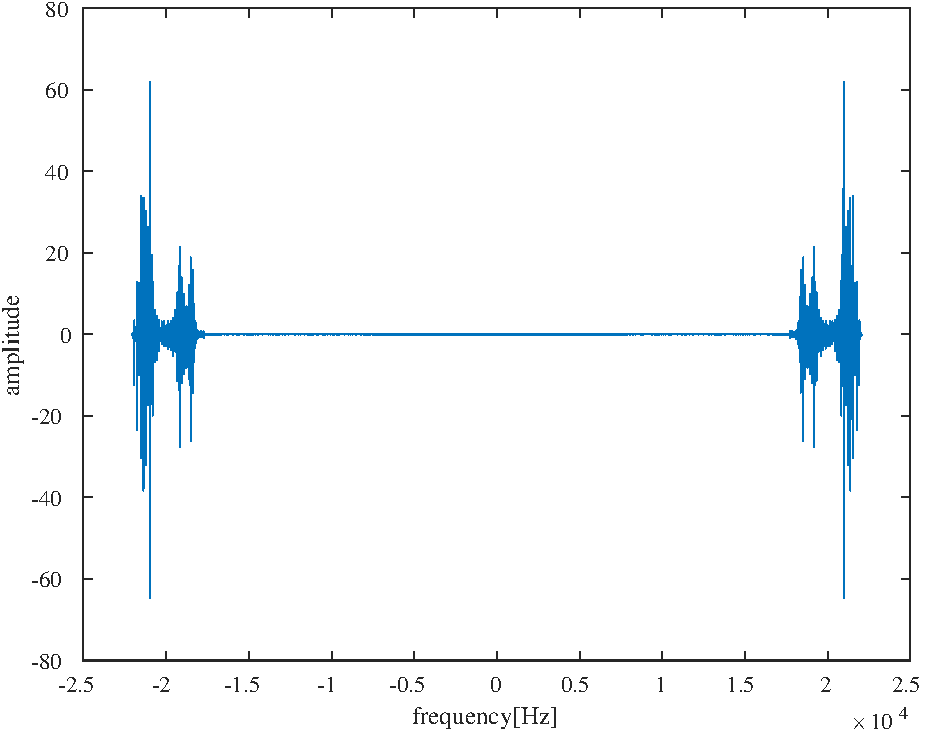
\includegraphics[keepaspectratio,width=.9\textwidth]{Figures/fft_fft.pdf}};
    \coordinate (figsouth) at (fig.south);
    \coordinate (figscenter) at ($(figsouth)+(2.75mm,7.1mm)$);
    \coordinate (figncenter) at ($(figscenter)+(0,5.48cm)$);
    \coordinate (figsleft) at ($(figscenter)+(-3.47cm,0)$);
    \coordinate (figsright) at ($(figscenter)+(3.47cm,0)$);
    \fill[fill=red,opacity=0.1](figsleft)--(figsleft |- figncenter)--(figncenter)--(figscenter)--cycle;
    \fill[fill=blue,opacity=0.1](figsright)--(figsright |- figncenter)--(figncenter)--(figscenter)--cycle;
    \coordinate (L) at($(figncenter)!0.5!(figsleft)+(0,1cm)$);
    \coordinate (R) at($(figncenter)!0.5!(figsright)+(0,1cm)$);
    \draw[very thick,dashed,latex-latex](L)to[bend left=40](R);
\end{tikzpicture}
        \caption{\texttt{fft}直後の出力データ}
        \label{fig:fft直後のデータ}
    \end{minipage}
    \begin{minipage}[b]{.48\textwidth}
        \centering
        \begin{tikzpicture}
    \node(fig){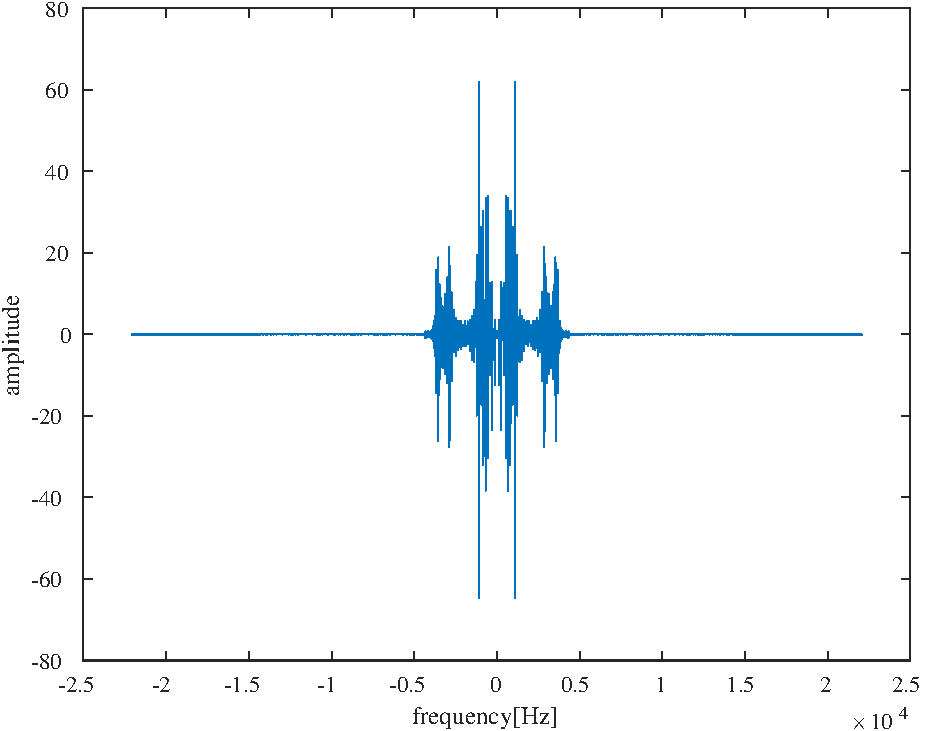
\includegraphics[keepaspectratio,width=.9\textwidth]{Figures/fft_fftshift.pdf}};
    \coordinate (figsouth) at (fig.south);
    \coordinate (figscenter) at ($(figsouth)+(2.75mm,7.1mm)$);
    \coordinate (figncenter) at ($(figscenter)+(0,5.48cm)$);
    \coordinate (figsleft) at ($(figscenter)+(-3.47cm,0)$);
    \coordinate (figsright) at ($(figscenter)+(3.47cm,0)$);
    \fill[fill=blue,opacity=0.1](figsleft)--(figsleft |- figncenter)--(figncenter)--(figscenter)--cycle;
    \fill[fill=red,opacity=0.1](figsright)--(figsright |- figncenter)--(figncenter)--(figscenter)--cycle;
\end{tikzpicture}
        \caption{\texttt{fftshift}後の出力データ}
        \label{fig:fftshift後のデータ}
    \end{minipage}\\
    \dotfill\\
    \begin{minipage}[b]{.48\textwidth}
        \centering
        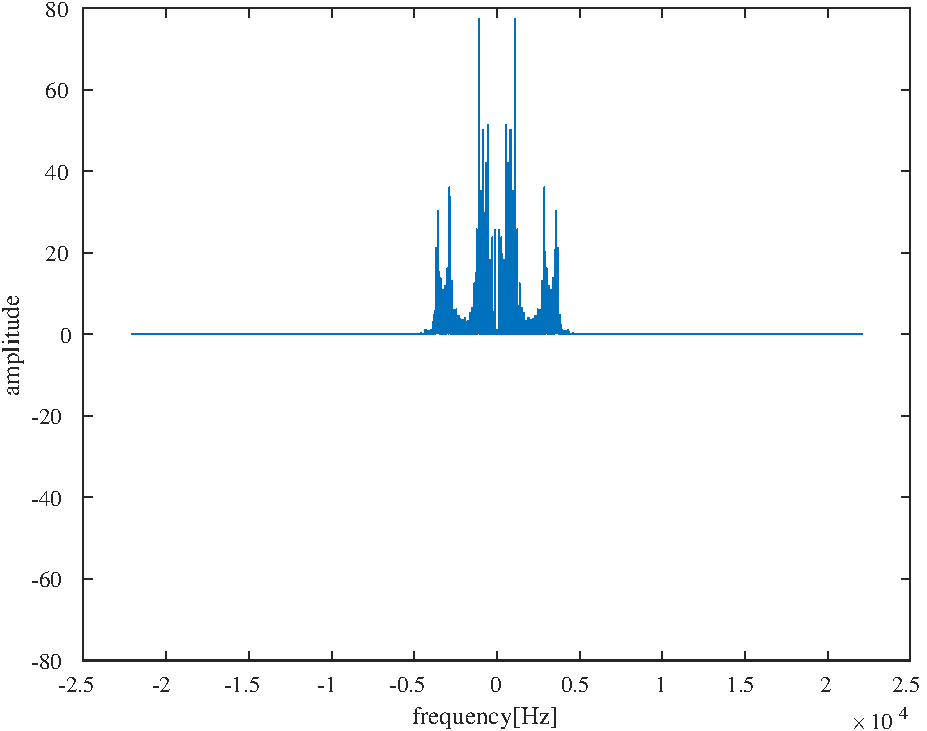
\includegraphics[keepaspectratio,width=.9\textwidth]{Figures/fft_abs.pdf}
        \caption{\texttt{abs}を適用した後のデータ(グラフ)}
        \label{fig:absを適用した後のデータ}
    \end{minipage}
    \begin{minipage}[b]{.48\textwidth}
        \centering
        \begin{lstlisting}[caption={振幅スペクトルの取得},label={src:振幅スペクトルの取得},numbers={none}]
y; % データ列
y_fft = fft(y); % 高速フーリエ変換
y_fftshift = fftshift(y_fft); % 左右交換
y_abs = fft_y; % 絶対値
ln = length(y_abs);
% 周波数テーブルの作成
freq = [-Fs/2 : Fs/ln : Fs/2 - Fs/ln];
plot(freq, y_abs); % グラフ描画
\end{lstlisting}
        \begin{flushleft}
            周波数テーブルの作成について,得られたデータ数\texttt{ln}に対して,
            周波数テーブルの長さ\texttt{Fs}に収める必要があるので,ステップ幅\texttt{Fs/ln}となる\texttt{-Fs/2}から\texttt{Fs/2}の配列を作成する.
        \end{flushleft}
    \end{minipage}
\end{figure}
\paragraph{実験の内容}今回の実験では,純音と矩形波の周波数解析する.サンプリング周波数を\(8192\textrm{Hz}\)と設定する.
\begin{figure}[H]
    \begin{minipage}[c]{.55\textwidth}
        \begin{itemize}
            \item[\textbf{純音}] \(440\textrm{Hz}\)の純音で実験する.
            \item 純音から\(1024\)点取り出す.\\
                  データ列の先頭から\(1024\)個のデータを選択する方法で行う.
            \item 振幅スペクトルを\(0\textrm{Hz}\)から\(1\textrm{kHz}\)まで描画する.
            \item \(440\textrm{Hz}\)にピークが来ているか確認する.
            \item[\textbf{矩形波}] \(128\)点値\(0\)が続き,\(128\)点値\(1\)が続く波形を\(4\)回繰り返す矩形波(\figref{fig:作成した矩形波}).
            \item 振幅スペクトルを\(0\textrm{Hz}\)から\(200\textrm{Hz}\)まで描画する.
            \item 高調波が発生しているか,その振幅が\eqref{equ:矩形波}通りになっているか確認する.
        \end{itemize}
        \scall\sref{src:02_01_1},\sref{src:02_01_2}.
    \end{minipage}
    \begin{minipage}[c]{.4\textwidth}
        \centering
        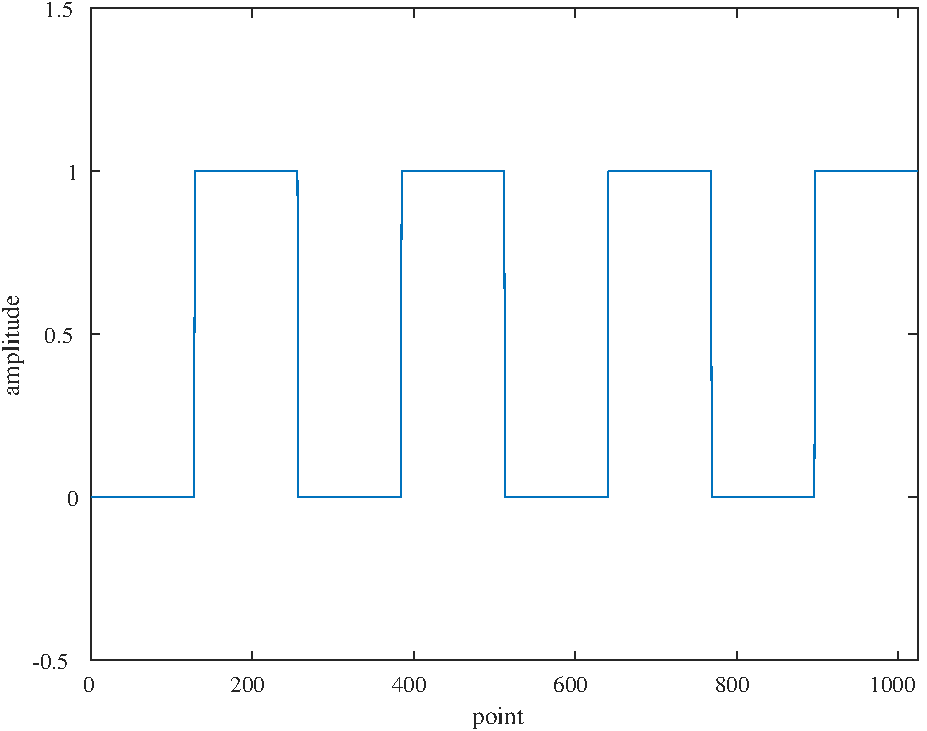
\includegraphics[keepaspectratio,width=\textwidth]{../../Figures/02_021.pdf}
        \caption{作成した矩形波}
        \label{fig:作成した矩形波}
    \end{minipage}
\end{figure}
\result
出力された結果に対して,特出する点の座標を表示させる.\figref{fig:\kadaiba_純音の振幅スペクトル}について,周波数\(440\textrm{Hz}\)の振幅は最大であることが分かった.
また,\figref{fig:\kadaiba_矩形波の振幅スペクトル}より図中にある点の高調波が確認された.
\begin{figure}[h]
    \centering
    \begin{minipage}{.48\textwidth}
        \centering
        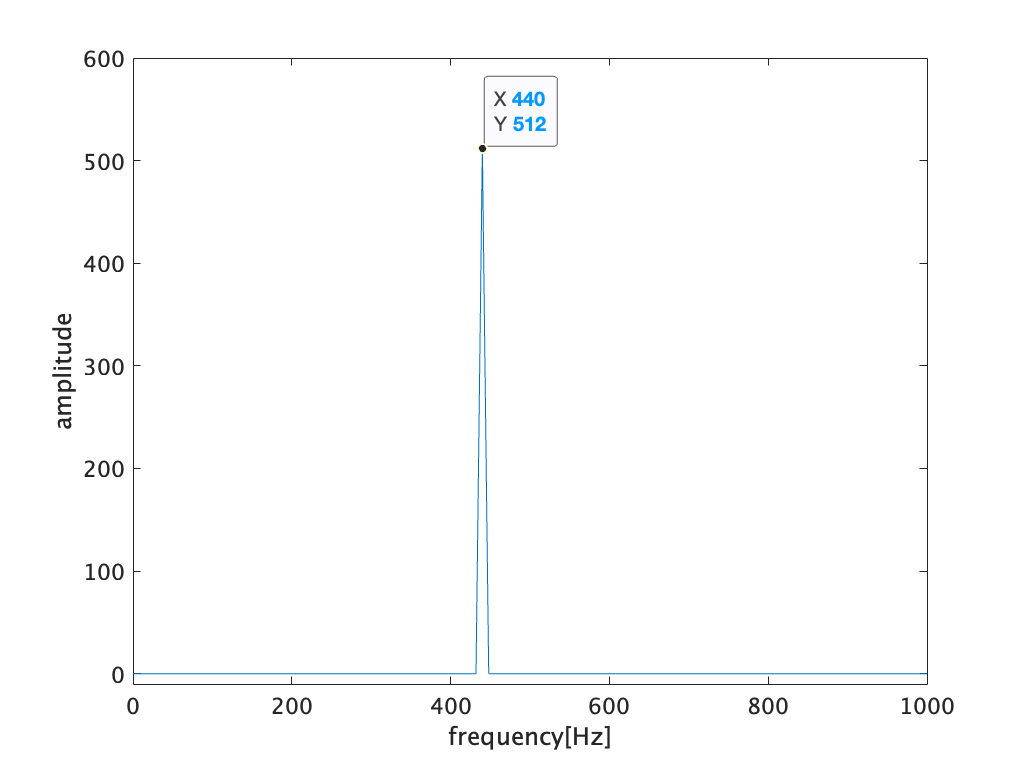
\includegraphics[keepaspectratio,width=\textwidth]{../../Figures/02_01.png}
        \caption{純音の振幅スペクトル}
        \label{fig:\kadaiba_純音の振幅スペクトル}
    \end{minipage}
    \begin{minipage}{.48\textwidth}
        \centering
        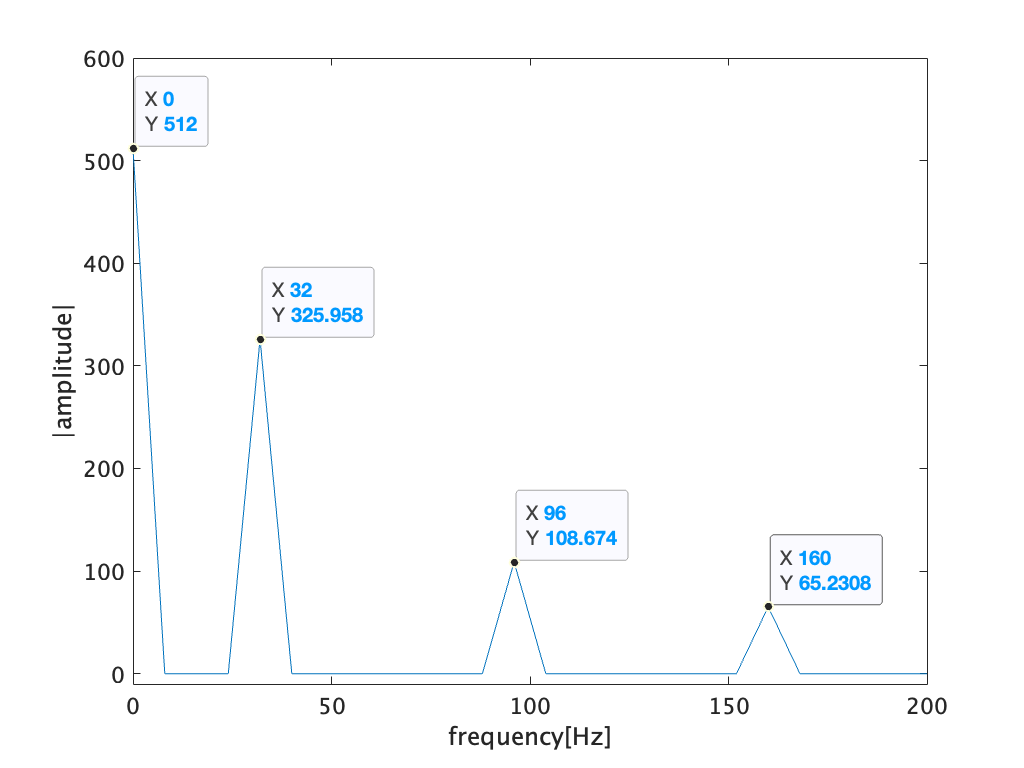
\includegraphics[keepaspectratio,width=\textwidth]{../../Figures/02_022.png}
        \caption{矩形波の振幅スペクトル}
        \label{fig:\kadaiba_矩形波の振幅スペクトル}
    \end{minipage}
\end{figure}
\consideration
\paragraph{純音}実験結果より,純音の周波数\(440\textrm{Hz}\)が一番多く,ほかの高調波は確認できなかった.
\paragraph{矩形波}\figref{fig:\kadaiba_矩形波の振幅スペクトル}より高調波の存在は確認できる.矩形波のフーリエ級数展開は\eqref{equ:矩形波}である.\(k=1,2,3\)のときの正弦波と,周波数\(X\),振幅\(Y\)を\eqref{equ:矩形波具体例}に示す.
\begin{equation}
    \begin{aligned}
        \sin(2\pi(2-1)ft)            & =\sin(2\pi ft)             & (k=1) &  & (X,Y) & =(32,325.958)  \\
        \frac{1}{3}\sin(2\pi(4-1)ft) & =\frac{1}{3}\sin(6\pi ft)  & (k=2) &  & (X,Y) & =(96,108.6474) \\
        \frac{1}{5}\sin(2\pi(6-1)ft) & =\frac{1}{5}\sin(10\pi ft) & (k=3) &  & (X,Y) & =(160,65.2308)
    \end{aligned}\label{equ:矩形波具体例}
\end{equation}
\((X,Y)=(0,512)\)の振幅スペクトルは直交成分であり,\(k=1\)を\((X,Y)=(32,325.958)\)とすると,振幅について,\(k=2,3\)の正弦波は,\(k=1\)の正弦波の\(108.674/325.958=1/3\)倍,\(65.2308/325.958=1/5\)倍であり,
周波数についても,\(k=2,3\)の正弦波は,\(k=1\)の正弦波の\(96/32=3\)倍,\(160/32=5/3\)倍になっている.これは\eqref{equ:矩形波具体例}の正弦波と一致する.
\section{\kadaibb}\label{sec:\kadaibb}
\purpose
ローパスフィルタ(以下LPF)は以下のように説明されている.
\begin{leftbar}
    ある周波数(カットオフ周波数)より高い周波数を通さないフィルタはLPF(ローパスフィルタ)と呼ばれる.\\\hfill\cite[p.65]{2019matlabで学ぶ実践画像}
\end{leftbar}
今回の実験ではLPFを作成して,別途作成した音に対してフィルタを適用する.
フィルタを適用する前後での振幅スペクトルを比較し,フィルタが機能しているかを確認するとともに,フィルタが適用されているか聴音確認する.
\method
今回フィルタを適用させる音源は,ドイツ語音階で「C4」から「C5」まで\(0.25\)秒ずつ音を提示する.提示する音の順序を\eqref{equ:音の順序}に,各音階の周波数を\tblref{tbl:音階と周波数}に示す.
\begin{align}
    \textrm{C4}\to\textrm{D4}\to\textrm{E4}\to\textrm{F4}\to\textrm{G4}\to\textrm{A4}\to\textrm{H4}\to\textrm{C5}\label{equ:音の順序}
\end{align}
音源に対して,G4より低い音のみを通過させるLPFを作成しフィルタを適用する.カットオフ周波数をG4の周波数に設定すると,G4の周波数より小さいわずかな成分が除去できないため,F4とG4の中間に位置する周波数(\(375\textrm{Hz}\))へ設定する.
\begin{table}[h]
    \centering
    \caption{音階と周波数}
    \label{tbl:音階と周波数}
    \begin{tabularx}{\textwidth}{ACCCCCCCC}
        \hline
        音階                 & C4     & D4     & E4     & F4     & G4     & A4     & H4     & C5     \\
        周波数\(\textrm{Hz}\) & 261.38 & 293.67 & 329.63 & 349.23 & 392.00 & 440.00 & 493.88 & 523.23 \\
        \hline
    \end{tabularx}
\end{table}
\paragraph{LPFの作成と適用}
今回はフィルタの行列を作る方法ではなく,周波数テーブルの閉区間\(\big[-375\textrm{Hz},375\textrm{Hz}\big]\)以外の振幅を\(0\)にする方法でフィルタを適用する.(\srcref{src:フィルターを適用する})\scall\sref{src:02_02}.
\begin{lstlisting}[caption={フィルターを適用する},label={src:フィルターを適用する},numbers={none}]
% データ列yをフーリエ変換後,ffthiftしてabsをとったものを "fft_y" に格納している.
% 周波数テーブルの変数名は "freq".
for k=1:length(fft_y)
    if freq(k) >= 375 || freq(k) <= -375
        fft_y(k) = 0;
    end
end
\end{lstlisting}
\result
LPF適用前の音声波形と,LPF適用後の音声波形をに示す.また,\figref{fig:振幅スペクトルの確認}には上図にフィルタ適用前の振幅スペクトル,下図にフィルタ適用後の振幅スペクトルを示している.聴音確認の結果G4以降の音は聞こえなかった.
\begin{figure}[h]
    \centering
    \begin{minipage}[b]{.3\textwidth}
        \centering
        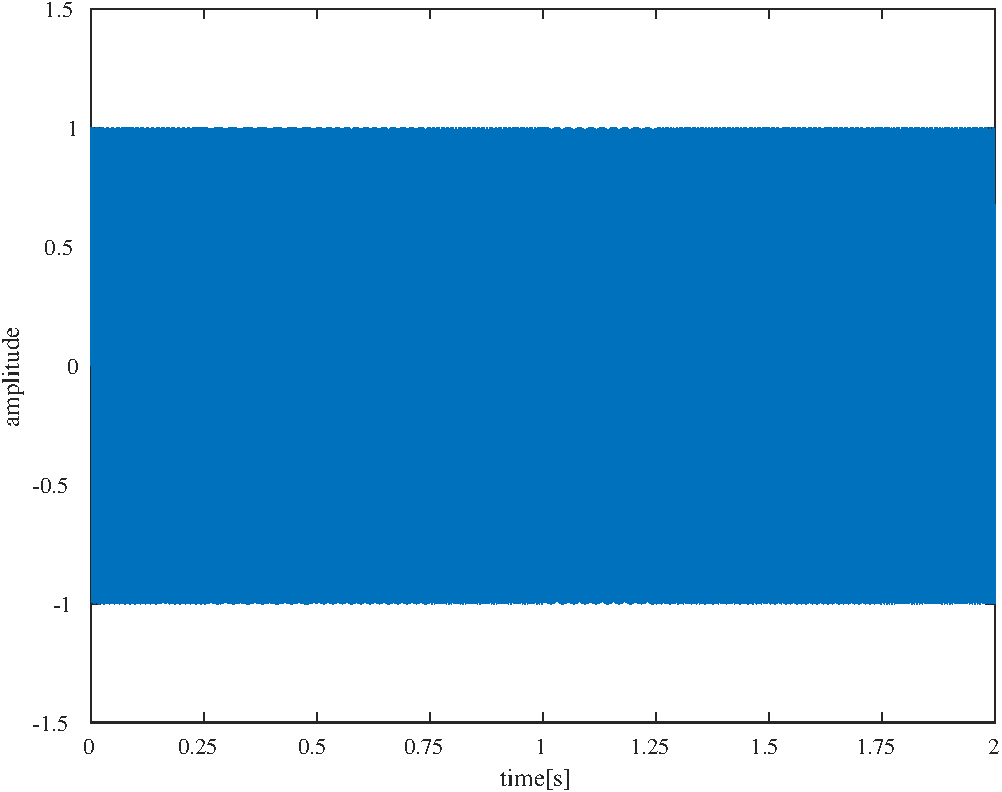
\includegraphics[keepaspectratio,width=\textwidth]{../../Figures/02_20.pdf}
        \caption{LPF適用前の波形}
        \label{fig:LPF適用前の波形}
    \end{minipage}
    \begin{minipage}[b]{.3\textwidth}
        \centering
        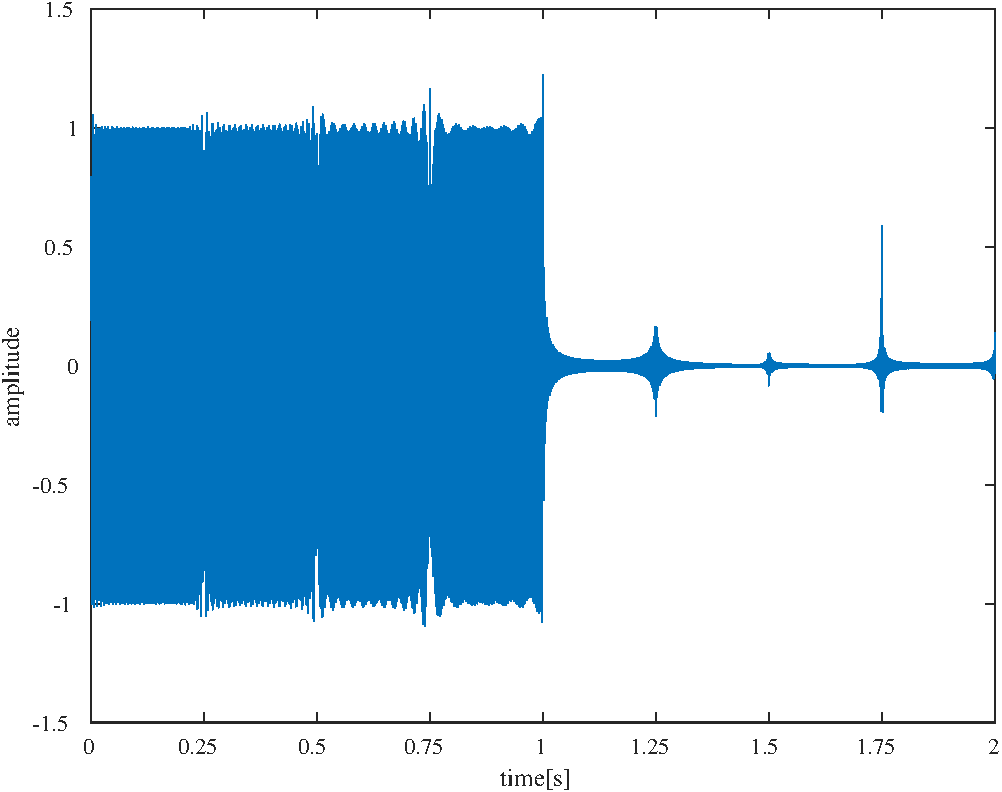
\includegraphics[keepaspectratio,width=\textwidth]{../../Figures/02_22.pdf}
        \caption{LPF適用後の波形}
        \label{fig:LPF適用後の波形}
    \end{minipage}
    \begin{minipage}[b]{.3\textwidth}
        \centering
        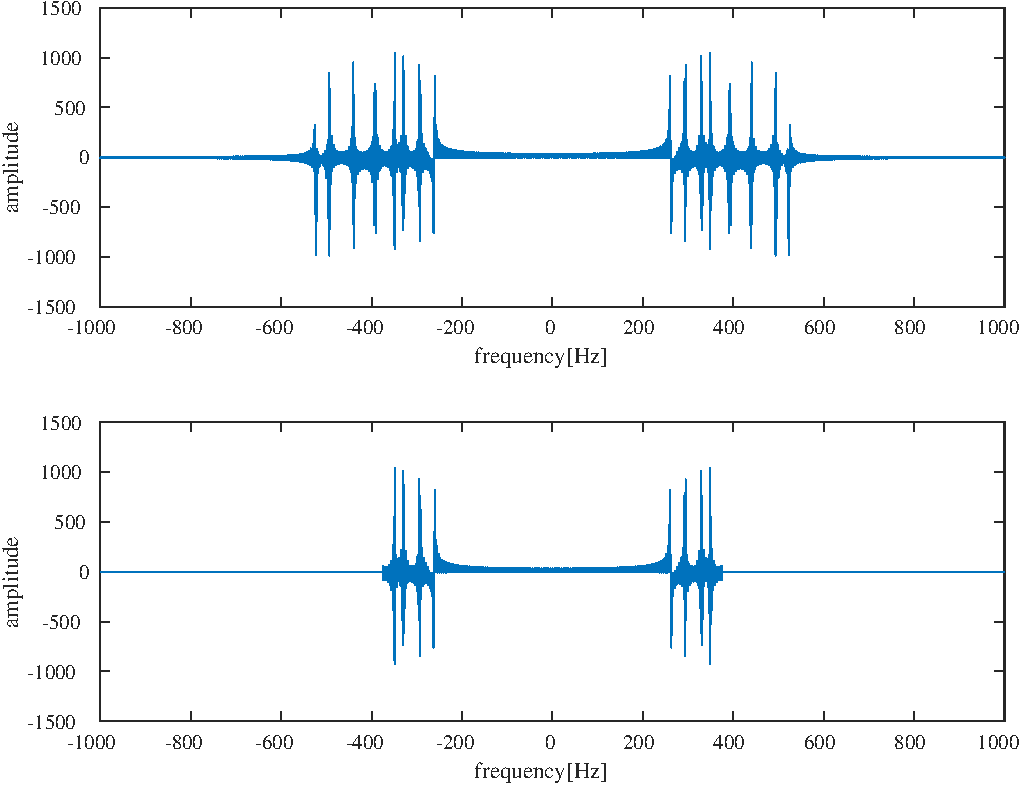
\includegraphics[keepaspectratio,width=\textwidth]{../../Figures/02_21.pdf}
        \caption{振幅スペクトルの確認}
        \label{fig:振幅スペクトルの確認}
    \end{minipage}
\end{figure}
\consideration
結果より\(1\)秒後の音以降が聞こえない.1音階\(0.25\)秒あるので,4音階分(C4,D4,E4,F4)までが聞こえることを考えると,実験結果は理論的に正しい.\figref{fig:振幅スペクトルの確認}より,特定周波数以降が切り取られていることも確認できる.
ただし,\(1\)秒後以降の波形も完全に0ではない理由は分からなかった.
